\documentclass{report}
\usepackage[utf8]{inputenc}
\usepackage{graphicx}
\usepackage{multirow}
\usepackage{minted}
\usepackage{listings}
\usepackage{algorithm}
\usepackage{algpseudocode}
\usepackage{hyperref}
\usepackage{biblatex}
\graphicspath{ {images/} }
\usepackage[a4paper, total={6in, 8in}]{geometry}

% Citations
\addbibresource{references.bib}

\title{\textbf{Genetic Programming as an Interpretable Alternative to Black-Box Machine Learning Models}}
\author{
    \textbf{Alexandros Georgousis}\\\\
    Candidate Number: 198828\\
    Supervisor: Dr. Christopher Buckley\\\\
    Department of Informatics\\
    BSc Computer Science
}
\date{May 2020}

\begin{document}

\begin{titlepage}
\maketitle
\end{titlepage}

\section*{Declaration}
This report is submitted as part requirement for the degree of BSc Computer Science at the University of Sussex. It is the product of my own labour except where indicated in the text. The report may be freely copied and distributed provided the source is acknowledged. I hereby give permission for a copy of this report to be loaned out to students in future years.\\

\noindent Signature:\\\\\\
Alexandros Georgousis

\clearpage

\section*{Acknowledgements}
I would like to thank Chris Buckley for his valuable insights and assistance with this project. I would also like to thank Martin Berger for his generous guidance during his time as my supervisor in the initial stages of the project, and his continuous support throughout its duration.

\begin{abstract}
Since the focus of AI research shifted from traditional programming approaches to Machine Learning, uninterpretability has been a big limitation of AI technologies. Recently, attempts have been made to incorporate some of these traditional approaches, such as Genetic Programming, into state-of-the-art AI research to tackle this problem. In this project, Genetic Programming is explored as a potential alternative to modern AI algorithms and is shown to produce interpretable solutions when applied directly to famous AI benchmark problems.
\end{abstract}
\clearpage

\tableofcontents
\listoffigures
\listoftables

\chapter{Introduction}
In the early days of AI, researchers utilised traditional programming techniques to simulate intelligent behaviour in machines. This meant that the ability of machines to perform complex tasks depended on the ability of humans to express solutions to those tasks in the form of precisely defined computational steps. This fundamental limitation led to the development of mathematical methods that allow programs to learn from experience, as opposed to following explicit instructions. These approaches are encapsulated in the field of Machine Learning (ML), which has risen to the forefront of AI research.

Recently, Neural Networks - a class of ML algorithms that loosely resemble the structure of biological neural networks in the brain - have gained a lot of popularity. Due to the growing availability of data and computational power, these algorithms have achieved comparable (and often superior) performance to humans at complicated tasks, from recognising faces to driving automobiles. One area in particular in which neural networks have shown extraordinary results is Reinforcement Learning (RL). RL is a technique in which a ML algorithm, called an agent, learns to operate in an environment (e.g. a video game) by interacting with it. The agent is allowed to operate freely in the environment, while trying to maximise some notion of a reward that its creators have defined.

Despite their usefulness, neural networks have important limitations. One such limitation is the issue of uninterpretability: the solutions produced by neural networks are too complicated for humans to understand. This problem is of particular importance in RL because our inability to understand an agent’s decision-making process makes it difficult to replicate desirable behaviours and prevent undesirable ones. Additionally, this problem presents an issue in morally significant situations. For example, imagine a medical AI tasked with diagnosing severe conditions in patients. Given its inability to explain its thought process, it would be difficult for patients to be convinced to make big life decisions based on the information they are given.

Many recent attempts have been made that used traditional AI techniques, such as Genetic Programming (GP), to tackle the problem of interpretability. GP is a technique that borrows concepts from biological evolution to automatically generate programs that solve a given problem. In most of these attempts, GP was used in combination with neural networks to produce solutions that perform well while, at the same time, offering a degree of interpretability. The limitation of these approaches is that uninterpretability cannot be eliminated as long as neural networks are part of the process. That’s why, in this project, GP was used directly as a standalone alternative to neural-network-based techniques, to produce solutions in the form of human-readable programs that achieve competitive performance in various RL tasks. 

The project began by applying GP to a simple classic control environment called cart-pole, in which the goal is to balance a wooden pole on a flat rectangular surface (figure \ref{fig:cart-pole}). I manually discovered a strategy for beating the game by interacting with the environment, and then I implemented a GP algorithm to automatically find a program that implements this strategy. After this experiment was successful, I wanted to apply the same algorithm to an environment that was similar enough to cart-pole but less constrained, and therefore more difficult to solve, to establish a baseline of problems of increasing difficulty that this algorithm would be able to tackle. So, I picked another popular ML benchmark called mountain-car, which simulates a vehicle attempting to climb a steep hill (figure \ref{fig:mountain-car}). I did not guide the algorithm to a known strategy this time, but instead implemented the required extensions to allow it to discover one by itself. The results were again positive: it was much easier for the algorithm to converge on a well-performing, and still interpretable, solution than I was expecting. Finally, I applied the algorithm on the inverted pendulum environment (figure \ref{fig:pendulum}), which needs to be swung until it points upwards and then balanced there for as long as possible. This environment is structurally similar to mountain-car, with the added difficulty of requiring to maintain the achieved state (pointing upwards) as opposed to simply reaching it. The GP algorithm managed to discover strategies that performed reasonably well and which, after being interpreted, were manually improved to eventually achieve performance close to the best neural-network-based solutions, without a loss in interpretability.

\begin{figure}[H]
    \centering
    \includegraphics[width=3.8cm]{images/cartpole}
    \caption{Cart-Pole}
    \label{fig:cart-pole}
\end{figure}

\begin{figure}[H]
    \centering
    \includegraphics[width=3.8cm]{images/mountain-car}
    \caption{Mountain-Car}
    \label{fig:mountain-car}
\end{figure}

\begin{figure}[H]
    \centering
    \includegraphics[width=3.8cm]{images/pendulum}
    \caption{Pendulum}
    \label{fig:pendulum}
\end{figure}

% \includegraphics[width=3.8cm]{cartpole.png}
% \includegraphics[width=3.8cm]{mountain-car.png}
% \includegraphics[width=3.8cm]{pendulum.png}

\section{Report Overview}
This report is structured in chapters. Chapter 1 includes the introduction and this overview section. Chapter 2 covers the professional considerations that need to be taken into account according to the BCS code of conduct. Chapter 3 provides background information on the technical topics relevant to the project, namely Machine Learning and Genetic Programming, as well as an overview of related work, and explains how the approach used in this project differs from other approaches. Chapter 4 discusses the methods used in the project, including details about the experiments performed and pseudocode to encourage replication. Chapters 5 and 6 cover the experiments performed using the RL environments (cart-pole, mountain-car, and pendulum, in that order) and the results obtained for each of them. Chapter 7 provides a conclusion as well as a discussion of the limitations of this project and suggestions for future extensions.

\chapter{Professional Considerations}
All third-party work that will be utilised to carry out this project, including academic papers and software tools, will be credited appropriately in this report\footnote{BCS Code of Conduct 1.b. “You shall have due regard for the legitimate rights of Third Parties.”}. All methods, source code, and results will be disclosed to encourage equal access to the benefits of this project.\footnote{BCS Code of Conduct 1.c. “You shall conduct your professional activities without discrimination on the grounds of sex, sexual orientation, marital status, nationality, colour, race, ethnic origin, religion, age or disability, or of any other condition or requirement.”}\footnote{BCS Code of Conduct 1.d. “You shall promote equal access to the benefits of IT and seek to promote the inclusion of all sectors in society wherever opportunities arise.”}\footnote{BCS Code of Conduct 4.f. “You shall encourage and support fellow members in their professional development.”} Finally, the work included in this project is directly related to my field of study as a Computer Science student and the assistance of qualified individuals will be requested where necessary\footnote{BCS Code of Conduct 2.a. “You shall only undertake to do work or provide a service that is within your professional competence.”}\footnote{BCS Code of Conduct 2.b. “You shall NOT claim any level of competence that you do not possess.”}.

\chapter{Background}
\section{Machine Learning}
Machine learning is a sub-field of AI, which studies the development of systems that learn from experience without being explicitly programmed. There are different machine learning approaches, including supervised, unsupervised, and reinforcement learning, which describe what information is provided to the system and the method by which it learns from that information. This section gives an overview of supervised and reinforcement learning, as well as the basics of neural networks and their interpretability limitations.

\subsection{Supervised Learning}
Supervised learning is the most popular and successful machine learning approach, in which an algorithm learns to solve a problem by being exposed to example solutions to that problem. Specifically, the algorithm is given a collection of inputs and corresponding outputs (labels). This collection is called training data and each input-output pair is called a training example. The algorithm, then, automatically infers a mapping between those inputs and outputs through a process called training, after which it is able to assign labels to inputs it has not seen before. Different algorithms use different training methods, and this section will focus on Neural Networks, one of the most popular class of such algorithms.

\subsection{Neural Networks}
A Neural Network (NN), is a ML algorithm used widely for supervised learning. This section provides an overview of the standard, feed-forward NN architecture, but note that there are various types of NNs with different architectures and methods of training.

\subsubsection{High-Level Representation}
Neural networks are commonly represented as a set of successive layers: one input layer, one or more hidden layers, and one output layer. Each of those layers consists of a set of nodes and each of those nodes is connected to every node of the successive layer. A graphical representation of this structure can be seen in figure \ref{fig:neural_network}. The nodes in the input layer of such a network represent the set of properties (features) that describe the object that the NN is meant to classify. For example, in the classic problem of recognising handwritten digits (see, for example, \cite{handwritten}) images of handwritten digits are 'shown' to the network, by assigning a numerical value to each pixel in an image and using those as features. Each node in the input layer, then, corresponds to one of those features. Every node in the input layer passes its value, along with a numerical weight that represents the significance of that value, to every node of the first hidden layer. Each node in a hidden layer represents a mathematical function, which performs an arithmetic operation on the inputs and weights it receives from the previous layer and produces an output, which it passes on to every node of the next layer, along with a new corresponding weight. This process repeats until the initial input values have propagated through and been manipulated by each of the hidden layers in succession. The values produced by the final hidden layer pass on to the output layer, which performs the final calculation before providing an output which represents the network prediction about the input it was shown. In the case of the handwritten digit recognition problem, there are 10 nodes in the output layer (one for each digit from 0-9), and the value of each node represents the network's confidence in the handwritten digit it was shown being the one represented by the corresponding node. The digit represented by the node with the highest value is chosen as the network's decision.

The goal of the training phase of a NN is to compute a set of weights such that the network makes as few wrong predictions as possible. The weights are initially set to arbitrary numerical values (usually random) and are slowly tuned to minimise the number of errors the NN makes. The result of this process is a set of optimal weights, which the NN can then use in the process described above to assign labels to inputs it has not seen before.

\begin{figure}[ht]
    \centering
    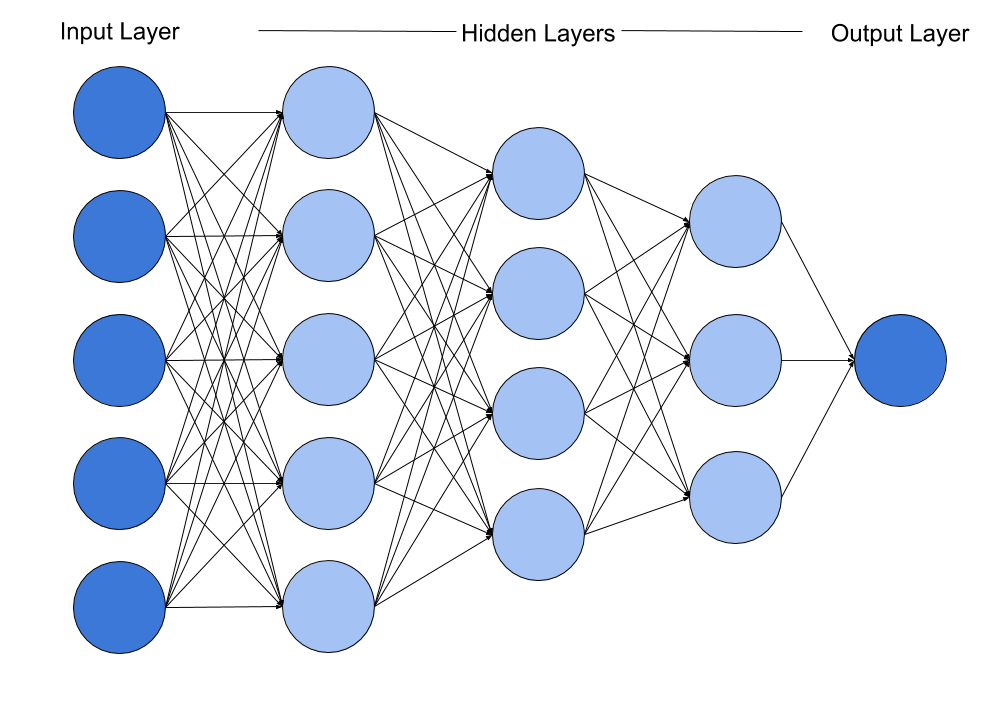
\includegraphics[width=12cm]{images/neural_network.png}
    \caption{Graphical representation of a feed-forward neural network with 3 hidden layers}
    \label{fig:neural_network}
\end{figure}

\subsection{Reinforcement Learning}
Reinforcement learning describes a process in which an algorithm (such as a neural network) plays the role of an agent that attempts to learn to operate in an environment by repeatedly interacting with it. The term "reinforcement" comes from the fact that the agent is provided with feedback from the environment, which comes in the form of a positive or negative reward depending on whether the agent is behaving in a way that brings it closer to achieving whatever goal the environment in question has set. The most intuitive example of such a setup is a video game, where the reward is the score the agent achieves by playing the game.

Similarly to supervised learning, the algorithm is provided with some input (the environment state) and learns to map it to some output (an action) such that some success metric (the reward) is optimised. However, in reinforcement learning, the algorithm is not provided with examples of correct input-output pairs. Instead, it has to actively interact with the environment to discover new inputs and learn to respond to them.

The process of reinforcement learning takes the form of an iterative experiment with some termination criteria. At the beginning of the experiment, the agent receives an encoded version of the initial state of the environment as input and outputs a random action, as it has no notion of which actions are going to yield maximum reward yet, which updates the state of the environment. Then, the environment provides the agent with a numerical reward (a positive or negative number representing reinforcement and punishment respectively) and the updated state. This process repeats until the agent achieves some predefined goal (e.g. wins the game) or one of the termination criteria is met (e.g. a timer runs out).

Like in supervised learning, neural networks are the most widely used algorithmic technique in reinforcement learning. In fact, the use of neural networks has given rise to a sub-field of reinforcement learning referred to as Deep Reinforcement Learning, which is characterised by the use of neural networks with multiple hidden layers.

\subsection{Uninterpretability of Machine Learning Models}
Since this project aims to propose a solution to the uninterpretability problem of current ML models, it is necessary to articulate clearly what uninterpretability means in this context and why these models suffer from it.

The simplest algorithm that is considered to belong to the set of ML models is linear regression. Linear regression is a statistical technique that attempts to infer a linear correlation between one or more variables. The result of applying this technique to a collection of concrete values for the variables in question is a linear model that "fits" the given data such that the error generated by predictions on the data using this model is minimal. The problem with this technique and, in fact, any statistical technique, is that it tells us nothing about the cause of the inferred relationship between the variables. That is to say, we know how the variables are correlated, but we don't know why that is, or what the exact relationship between them is. Take the popular problem of predicting house prices \cite{housing} as an example. Given a set of house characteristics along with the price each house was sold for, a model can be trained to predict the prices of houses it has not seen before. However, the model can tell us nothing about why, say, increasing the number of bedrooms tends to be correlated with an increase in price; it can merely tell us that, based on the available data, this seems to be the case. 

Neural networks are essentially more complex versions of traditional statistical techniques. This added complexity only serves to compound the problem of uninterpretability by increasing the number of transformations the original data undergoes to produce predictions, as well as the number of parameters the model requires to tune to make those predictions more accurate. Put simply, the only information the model provides us with is a table of floating-point numbers and a series of algebraic calculations that produce the prediction. This makes it impossible for humans to understand the reasoning behind the "decisions" a neural network makes, since they always take the form of statistical predictions. 

We might often be tempted to attribute reasoning to neural networks that perform high-level tasks, such as a neural network learning to play a video game via reinforcement learning, but this is an illusion: all the network does is receive encoded inputs, perform some calculations on them, and output the result, which the neural network predicts will produce an action in the video game that will bring it closer to the predefined "win" condition.

\section{Genetic Programming}
Genetic programming (GP) is a technique that borrows concepts from biological evolution to automatically generate programs that solve a specific problem. The algorithm generates an initial population of random programs and progressively modifies them until a program that can solve the problem in question emerges. GP takes the form of an iterative process in which the programs are repeatedly evaluated using a procedure (fitness function) to compute a measure of their performance. Then, a set of operations called genetic operations are performed on the population to produce a new generation of programs that are likely to perform better than their predecessors.

The characteristics of GP algorithms can be mapped to the components of a reinforcement learning agent to allow GP to be used on reinforcement learning tasks. Specifically, programs in a population can take the form of functions that take an environment state as input and produce an action as output. Subsequently, the reward provided by the environment can be used as the fitness measure for the programs, using which the algorithm can pick programs that perform well and discard the ones who don't. This mapping makes it possible to apply GP to reinforcement learning tasks.

\subsection{Program Structure}
In order to generate programs, the GP algorithm uses a domain-specific language (DSL) which is a language designed with the characteristics of the given problem in mind, as opposed to a general-purpose language which is designed to describe programs for any problem. The DSL consists of a function set and a terminal set. The function set contains the names of all the functions that can be used to construct programs and the terminal set contains variables and constants (terminals) that can be given as inputs to these functions. 

In the case of a typed DSL, each function takes a fixed number of arguments, each of which has to be of a specific type (e.g. 'number' or 'string'). The amount of arguments a function takes is known as its arity. Therefore, when constructing programs using this language, the GP algorithm has to ensure that the number of terminals chosen as the arguments to a function matches its arity, and that the type of each terminal matches that of the corresponding argument. If a function produces an output, then that also has a type, which must be checked when a function is passed as an argument to another function. If the DSL is untyped, any function can take any terminal or other function as an argument without any restrictions.

\subsection{Tree-Based Program Representation}
Programs generated by a GP algorithm can be represented as trees. The root (top) node of the tree represents a function, and each of its branches represents an argument to that function. If a branch leads to a node with more branches (sub-tree), then this is also a function. Eventually, every sub-tree has to reach a node that has no branches, called a leaf, and each leaf represents a terminal (e.g. a number) that is passed as an argument to the function represented by the root of the sub-tree that leaf is connected to. For example, figure \ref{fig:example_program_tree} shows a visual representation of a program that consists of a function, \verb+IFLTE+ (if-less-than-or-equal), which takes four arguments: three terminals (\verb+pa+, \verb+0+, and \verb+R+) and another \verb+IFLTE+ function which takes four terminals (\verb+pv+, \verb+0+, \verb+L+, and \verb+R+) as its arguments.

\begin{figure}[ht]
    \centering
    
\includegraphics[width=10cm]{images/complex_iflte_program.png}
    \caption{Tree representation of an example program produced by a GP algorithm.}
    \label{fig:example_program_tree}
\end{figure}

\subsection{Genetic Operators}
Genetic operators are algorithms that take one or more programs from a population as input and generate a new program as output. The three main types of genetic operators are selection, mutation and crossover. Selection is the simplest of the three and is commonly used to pick programs from the population to be used by the other two operators. There are many different selection algorithms, two of the most popular being fitness proportionate selection (aka roulette wheel selection) and tournament selection. Fitness proportionate selection uses a pseudorandom number generator to select programs from a population such that the higher the fitness of a program, the higher the probability that program will be chosen. Tournament selection randomly selects a subset of the programs in a population (the size of the subset is called tournament size) and picks the program with the highest fitness; the higher a program's fitness, the higher its probability of "winning" any of the tournaments it's placed in. Tournament selection provides more flexibility than fitness proportionate selection because it's possible to adjust the probability of weak individuals being selected (selection pressure) by increasing or decreasing the tournament size. Decreasing the selection pressure can be useful to avoid early convergence, i.e. the fittest programs of the first few generations dominating the population and not allowing better programs to emerge.

The mutation operator randomly selects a proportion of the programs in the population, and changes one of the program's sub-trees (in the case of tree-based representation) with a randomly generated sub-tree. The exact value of the proportion of the population that is selected for mutation is called the mutation rate of the algorithm.

Finally, crossover attempts to simulate a simple version of biological sexual reproduction. It selects two programs (parents) from the population using the selection operator, randomly picks a node on each of them (crossover point) and then combines the sub-trees that have the chosen node as their root to create a new program (offspring). The proportion of programs generated using crossover is called the crossover rate. Crossover was not used in this project for the sake of simplicity, as it did not prove necessary for the generation of programs that served as good solutions to the problems tackled.

\section{Related Work}
The problem of the uninterpretability of ML models has been known for a long time and a lot of research has been done to address the issue. Additionally, Genetic Programming has been a useful optimisation technique since its establishment with papers such as \cite{koza}, from which this project borrowed the idea for the \verb+IFLTE+ function, which served as the primary building block for the solutions produced and discussed in this report. Recently, there have been quite a few attempts to integrate Genetic Algorithms (of which GP algorithms are a subset) into the ML workflow, as seen for example in \cite{relatedwork1}, \cite{relatedwork2} and \cite{relatedwork3}, as well as attempts to use GP (e.g. \cite{gprl}, \cite{pirl}, \cite{atari}) to make solutions to ML problems more interpretable. To my knowledge, however, all of these approaches either use neural networks in some fashion, thus inevitably trading interpretability for performance, or use GP as a black-box algorithm whose solutions are no more interpretable than those produced by a neural network.

In this project, GP was used directly to attempt to solve problems that are traditionally solved using black-box ML models. The solutions produced take the form of human-readable programs that use familiar logical structures and high-level representations of the problem parameters to make them interpretable. The hope is that this will allow us to reason about solutions to these problems, instead of merely relying on the robustness of the black-box models that produce them.

\chapter{Methods}
This project aims to investigate the suitability of GP for solving modern AI problems. To this end, a GP algorithm was implemented and trained on a few chosen RL environments, and experiments were conducted to evaluate its performance. The purpose of this chapter is to provide an overview of the general structure of the RL environments used in this project, cover the details of the GP algorithm implemented to solve them, and serve as a guide for replicating the results discussed in the following chapters.

%%%%%%%%%%%%%%%%%%%%%%%%
% 4.1 Gym Environments %
%%%%%%%%%%%%%%%%%%%%%%%%

\section{RL Environments}
The RL environments used in this project were implemented by OpenAI and are publicly available in their open-source gym library\footnote{\url{https://gym.openai.com/}}. The library offers a simple API for running an environment as a simulation (see code snippet in figure 4.1), following the reinforcement learning loop described in the relevant Background section. For the simulation to start, the environment needs to be reset, a process which generates the initial state (observation) of the environment. The simulation can then start running for, at most, a predefined number of time-steps or until one of the termination criteria is met. On each step, a value which is interpreted as the action the agent wishes to take, must be passed to the environment. This value must belong to the action space defined by the environment for it to be considered valid. After the action is received by the environment, its internal state is updated accordingly and the corresponding observation object is returned to the agent, along with a numerical value which represents the reward, and a boolean value indicating whether any of the termination criteria have been met. The last component of these environments is a solution criterion, a condition in which they are considered "solved". The solution criteria for each of the environments discussed in this report are mentioned at the beginning of each corresponding chapter.

\begin{figure}[ht]
    \centering
    \begin{minted}[linenos]{python}
    import gym
    
    env = gym.make('CartPole-v0')
    obs = env.reset()
    done = False
    
    while not done:
        env.render()
        # Take a random action
        action = env.action_space.sample()
        obs, reward, done, _ = env.step(action)
    env.close()
    \end{minted}
    \caption{Implementation of a random agent for the cart-pole environment}
    \label{fig:simple_gym_env}
\end{figure}


%%%%%%%%%%%%%%%%%%%%%%%%%%%
% 4.2 Genetic Programming %
%%%%%%%%%%%%%%%%%%%%%%%%%%%

\section{Genetic Programming}
\subsection{Program Structure}
The DSL designed for the GP algorithm is a simple typed functional language. The function and terminal sets were made flexible to be able to be adapted to the RL environment the language was used for. Regardless of the specific functions and terminals used, however, the program structure remained the same. Each program is a function that takes the environment state as input and outputs an action to be taken in the next time-step in the environment. The simplest program in this language consists of a single terminal and, therefore, represents an agent that constantly takes a single action, regardless of the environment state. 

\subsection{Program Representation}
In this implementation of GP, programs are represented as trees, where each node is either a function or a constant and the branches represent a function-input relationship between the two nodes they connect (this is described in detail in the relevant Background section). In the project, these trees were implemented as Python lists. The first element of such a list is the name of a function (the root of the tree) as a string. The remaining elements of the list are the inputs to that function and they can be lists themselves (sub-trees) or the string representation of the terminal they encode. For example, the list representation of the tree depicted in figure \ref{fig:example_program_tree} would be:

\begin{verbatim}
["IFLTE", "pa", "0", ["IFLTE", "pv", "0", "L", "R"], "R"]
\end{verbatim}

For the sake of readability, a string representation of programs was implemented. In this representation, the program represented as a list above would be:

\begin{verbatim}
"IFLTE(pa, 0, IFLTE(pv, 0, L, R), R)"
\end{verbatim}

This representation looks much more like the functional programming style of syntax that these programs were meant to follow.

\subsection{Algorithm Details}
The pseudocode for the main GP algorithm is shown in Algorithm 1. The inputs to the algorithm are the size of the population, the maximum number of generations that can be evolved before termination, the termination fitness, and the mutation rate. The algorithm first creates an initial population of randomly generated programs. Next, it iteratively computes the fitness of each program in the population, uses the computed fitness scores to select programs to form the next generation (the same program can be selected more than once), applies mutation to the selected programs, gets the best program (highest fitness) from the new population, and updates the generation counter. This loop terminates if the maximum number of generations has been reached or if the best program has a fitness score greater than or equal to the termination fitness score. Once the loop terminates, the algorithm outputs the last recorded best program and exits.

\begin{algorithm}[ht]
	\caption{GP}
	\textbf{Inputs:} pop\_size, max\_gens, term\_fitness, mutation\_rate
	\begin{algorithmic}[1]
	    \State best\_program $\leftarrow$ NULL
	    \State population $\leftarrow$ gen\_init\_pop(pop\_size)
	    \Repeat
	        \State population\_fitness $\leftarrow$ fitness(population)
	        \State selected $\leftarrow$ select(population, pop\_size, population\_fitness)
	        \State mutate(selected, mutation\_rate)
	        \State population $\leftarrow$ selected
	        \State best\_program $\leftarrow$ best(population, population\_fitness)
	        \State gen $\leftarrow$ gen + 1
	    \Until gen $\geq$ max\_gens \textbf{or} fitness(best\_program) $\geq$ term\_fitness
	\end{algorithmic}
	\textbf{Output:} best\_program
\end{algorithm}

\subsubsection{Fitness Function}
The fitness function is the point of intersection between the GP algorithm and the RL environments. For the fitness of a program in the population to be computed, a gym environment has to be set up. The program is used to decide the action that is passed to the \verb+step+ function of the environment object (line 11 in figure \ref{fig:simple_gym_env}). Specifically, the interpreter implemented for the DSL is called with the program in question as input, and the output returned by the interpreter is passed to the step function. The fitness of the program is the average reward collected during the environment run.

\section{Performance Evaluation}
For each of the environments the GP algorithm was trained on, experiments were performed to evaluate the algorithm's performance. All experiments followed a similar structure so that the results would be comparable across different environments and different versions of the algorithm, to assess the effect of any modifications meaningfully. 

Each experiment was described by a set of parameters which were used to tune various properties of the GP algorithm and of the experiment itself. These parameters included the population size, the maximum number of generations the algorithm would evolve before terminating, the maximum fitness it would attempt to achieve (terminal fitness), and the maximum program depth, mutation rate and tournament size. Not all of these parameters were used in every experiment, as some depended on the complexity of the program structure and specific components of the algorithm that were not used in some experiments. Finally, the number of times the experiment would be performed had to be defined to average the results over multiple instances (runs) of the experiment, to make the results more robust.

The results that were recorded during each experiment were (1) the average fitness achieved by each generation of programs, (2) the fitness of the best-performing program of the last generation (which should, on average, be the best-performing program of the entire GP run), and (3) the best-performing program itself. (1) was used to produce a graph to visually represent the rate of improvement of the algorithm across all generations, which would provide useful information, such as the rate of convergence, for assessing the algorithm's performance and diagnosing problems, such as early convergence. (2) defined a metric for the overall performance of the algorithm and was used to assess improvement (or lack thereof) as well as compare the results achieved here with publicly available results on the same environments, particularly ones that use popular neural-network-based algorithms. Finally, (3) was analysed to assess the interpretability of the strategies produced by the GP algorithm, as well as to reason about potential modifications to the program structure that could improve performance.

\chapter{Cart-Pole \& Mountain-Car}
\section{Cart-Pole}
The cart-pole environment, which is an implementation of the famous cart-pole problem [7], is a popular AI benchmark that simulates a pole that needs to be balanced on the flat rectangle (cart) that it's attached to. The observation object of this environment includes the velocity and position of the cart, the velocity at the tip of the pole, and the angle of the pole. Initially, these parameters are assigned a random value in the range $[-0.05, 0.05]$, which results in the pole standing almost upright with a slight tilt. The environment only allows two discrete actions (left and right) which the agent uses to balance the pole before it falls over, by pushing the cart without causing it to go off-screen. The environment terminates if the agent fails in either of those tasks, or after the maximum number of time-steps (200) is reached. The agent receives $1$ reward on every time-step until one of these termination criteria is met. Finally, this environment is considered to be solved if the agent achieves an average reward of greater than or equal to $195.0$ over 100 consecutive trials. More details about the various environmental parameters can be found in the environment’s official GitHub Wiki page\footnote{\url{https://github.com/openai/gym/wiki/CartPole-v0}}.

\subsection{Experiment 1: Binary Programs}
The goal of the first experiment was to implement the simplest GP algorithm that performs better than a random agent. The simplest language that can encode the actions allowed in this environment is one of 0’s and 1’s, where 0’s represent ‘left’ and 1’s represent ‘right’. The program structure, therefore, included the terminal set \verb+T = {0, 1}+ and an empty function set. The intuition for this structure was that, in principle, there has to exist a string of left-right actions that manages to balance the pole on the cart most of the time. 

This GP agent did not managed to achieve better-than-random performance: a random agent achieves an average reward of $\approx22.0$ and the best programs the GP algorithm generated achieved an average reward of $16.76$. The most likely reason for this is that these programs are static, which means they don’t use information about the state of the environment to compute the next action to take. This limitation would not be a problem if the initial state of the environment was always the same, because that would make the state transitions deterministic and, therefore, there would exist a static program that would reliably balance the pole. However, the initial state of the environment is randomised each time the environment starts running and the range of possible values for the various parameters of the environment is sufficiently large, such that no static strategy can perform well.

\subsection{Experiment 2: Known Strategy}
The main goal of the second experiment was to enable the agent to utilise the environment state to choose actions dynamically. At the same time, I wanted to test the capabilities of the GP algorithm, since it would be used to find increasingly complex programs as the environments proved to be more difficult to solve. To achieve both of these goals, a manual strategy was discovered that performed well by utilising the environment state. The program structure of the GP algorithm was also adjusted to allow it to discover the strategy automatically. The chosen strategy can be described as follows:

\begin{verbatim}
    if pole_angle <= 0 then push_left() else push_right()
\end{verbatim}

Intuitively, this strategy describes the behaviour "if the pole is leaning to the left, push the cart to the left; if the pole is leaning to the right, push the cart to the right". This should keep the pole balanced at all times. To test this intuition, I implemented an agent that follows this strategy and tested it on the environment. The agent achieved an average score of $42.0$, a major improvement over the previous agent. Then, I introduced a simple environment-specific language to replace the binary language of the previous experiment, which included variables to represent the environment state and the actions the agent can take, flow-control (if-statements) and comparison operators to allow the agent to make decisions dynamically, and constants for calculations. The function and terminal set used for this experiment were \verb+F = {IFLTE}+ and \verb+T = {pa, 0, L, R}+ respectively.

The function set included a single function, \verb+IFLTE+ (if-less-than-or-equal), which accepts 4 inputs; if the first input is less than or equal to the second input, it outputs the third input; otherwise, it outputs the fourth input. This functionality seemed sufficient to encode the strategy described above. The terminal set included four elements: the pole angle (\verb+pa+) used to encode the corresponding environment observation, the numerical constant \verb+0+ which was required for the comparison performed in the strategy, and the actions \verb+L+ and \verb+R+, left and right respectively. The program structure was quite restricted in this first version of the algorithm to make it easier to evaluate and troubleshoot before applying it to more difficult environments that would require a more complex program structure. Specifically, each program was restricted to consist of a single \verb+IFLTE+ function, which could only accept \verb+pa+ and \verb+0+ as its first two arguments, and \verb+L+ and \verb+R+ as its third and fourth arguments (figure \ref{fig:iflte_tree}). It was important to restrict the third and fourth arguments to actions since the output of the program had to be the action the agent would perform in the environment. Therefore, a simple type system was implemented to perform this check. Using this simple functional language, the manually-discovered strategy could be encoded as \verb+IFLTE(pa, 0, L, R)+.

\begin{figure}[ht]
    \centering
    
\includegraphics[width=12cm]{images/simple_iflte_program.png}
    \caption{Tree representation of the program structure of the Known Strategy agent}
    \label{fig:iflte_tree}
\end{figure}

With these structural restrictions, it was easy for the GP algorithm to converge to the intended strategy (it only required a single generation, and mutation was not needed) because the program space was very small. The exact parameters used for the experiment are summarised in table \ref{tab:cartpole_exp2_params}.

\begin{table}[ht]
    \centering
    \begin{tabular}{|l|c|}
        \hline
        \textbf{Parameters} & \textbf{Values} \\
        \hline
        Population size     & 10  \\
        Max generations     & 5   \\
        Max program depth   & 1  \\
        Terminal fitness & 195.0 \\
        Number of runs      & 1   \\
        Number of episodes  & 100 \\
        Episode length      & 200  \\
        \hline
    \end{tabular}
    \caption{Experiment parameters (cart-pole experiment 2)}
    \label{tab:cartpole_exp2_params}
\end{table}

\subsection{Experiment 3: Exploration}
\subsubsection{Setup and Motivation}
The goal of the final experiment was to expand the program space to encourage exploration and allow the algorithm to discover better strategies than the one found manually. The terminal set was extended to include the second observation of the environment, pole velocity (\verb+pv+), to allow the algorithm to incorporate it in the solution. Additionally, I experimented with constants other than \verb+0+ and it turned out that the performance was very sensitive to even very small deviations from \verb+0+. Specifically, I discovered that including the constant \verb+0.025+ in the terminal set increased the performance of the discovered solutions significantly. Finally, the program structure was adapted to allow for the generation of programs that utilised higher-order functions (i.e. functions that accept functions as arguments) which can be represented as a trees of varying depth (see figure \ref{fig:deep_iflte_tree} for an example). The extended terminal set was \verb+T = {pa, pv, 0, 0.025, L, R}+. The parameters used for this experiment are summarised in table \ref{tab:cartpole_exp3_params}.

\begin{figure}[ht]
    \centering
    
\includegraphics[width=12cm]{images/complex_iflte_program.png}
    \caption{Tree representation of the program structure of the Exploration agent}
    \label{fig:deep_iflte_tree}
\end{figure}

\begin{table}[ht]
    \centering
    \begin{tabular}{|l|c|}
        \hline
        \textbf{Parameters} & \textbf{Values} \\
        \hline
        Population size     & 100  \\
        Max generations     & 5  \\
        Max program depth   & 2  \\
        Terminal fitness & 195.0 \\
        Number of runs      & 1   \\
        Number of episodes  & 100 \\
        Episode length      & 200  \\
        \hline
    \end{tabular}
    \caption{Experiment parameters (cart-pole experiment 3)}
    \label{tab:cartpole_exp3_params}
\end{table}

\subsubsection{Results and Discussion}
The initial results of this experiment showed that the second observation, pole velocity, was more useful than the pole angle, so programs using \verb+pv+ instead of \verb+pa+ tended to dominate the population during the first few generations. The first run of GP converged on the program \verb+IFLTE(pv, 0, L, R)+, which achieved an average reward of $181.78$. This improvement could be attributed to the fact that the velocity of the pole provided the agent with more useful information than its angle. Using the first strategy (\verb+IFLTE(pa, 0, L, R)+), if the pole leaned towards, say, the right at the beginning of the run, the agent would begin to push the cart to the right to cause the pole to lean towards the left, bringing it back to the center. The problem with this strategy was that by the time the pole angle became negative (meaning the pole leaned towards the left) it had accumulated too much momentum for the agent to manage to push left to balance it on time. The agent was essentially over-correcting. Using the new strategy, the agent detected which direction the pole was accelerating towards (using the sign of its velocity) and pushed the cart towards that direction for just long enough to prevent the pole from falling over, without over-correcting. However, this strategy was still problematic (as is evident from the imperfect score it achieved) because the agent stopped pushing the cart as soon as the sign of the pole velocity was flipped, so the pole didn't have enough momentum to lean towards the other side, thereby letting it fall towards the same side again. The result of this was that the agent was now under-correcting, balancing the pole perfectly, but at an angle, causing the cart to move until it eventually exited the screen and the environment terminated. It was evident at this point that a solution would involve information about both the pole angle and its velocity.

Increasing the maximum number of generations from 5 to 10 allowed for more complex solutions to arise. Eventually, the algorithm consistently produced solutions that achieved the reward specified as the solution criterion for the environment. These solutions included programs using nested if statements and combining both observation variables. An example of such a program is:
\begin{verbatim}IFLTE(0.025, pa, IFLTE(pv, pv, R, L), IFLTE(0.025, pv, R, L))\end{verbatim}
This program achieves an average reward of $198.74$ over 100 consecutive trials. The following is an equivalent, but more readable, version of the strategy described by this program:

\begin{verbatim}
if pa > 0.025 then R else (if pv > 0.025 then R else L)
\end{verbatim}

Following this strategy, the agent pushed the cart to the right to balance the pole if it was leaning at a right angle greater than some threshold ($0.025$). If the pole was leaning at a left angle or a small right angle, the agent checked the pole's velocity to make its decision: if the pole was accelerating towards the right (\verb+pv > 0.025+) then the agent pushed right to counteract it; otherwise it pushed left for the same reason.

This extended version of the program structure allowed the agent to achieve the goal of utilising exploration to find new and better solutions by exploring a larger program space. At this stage, the GP algorithm can incorporate new language extensions as well as additional genetic operators, both of which will be required in the following environments. So, Cart Pole was a useful starting point in showcasing the potential of this approach and establishing a framework for applying it to other RL environments.

\section{Mountain-Car}
The second RL environment attempted, was mountain-car. This environment simulates a car that attempts to climb a steep hill (figure \ref{fig:mountain-car}). There are two versions of this environment, one in which the actions the agent can take are discrete (similar to cart-pole) and one in which they are continuous (the action is a number that represents the magnitude of the force the agent applies to the car). The former is, in principle, easier to solve because there are fewer possible actions and, therefore, fewer strategies to explore before discovering a solution. The discrete version of the environment was attempted first with the hope that a solution to the simpler environment could be used as a basis for the more complex one.

\subsection{Experiment 1: Discrete Actions}
For the discrete version of this environment, I used the same parameters as in cart-pole experiment 3, and a similar program structure, adapted to the details of this environment:

\begin{verbatim}
F = {IFLTE}
T = {position, velocity, 0.0, 0, 1, 2}
\end{verbatim}
The terminals \verb+position+ and \verb+velocity+ represent the corresponding environment observations, \verb+0.0+ is a numerical constant used for comparisons (similar to cart-pole), and \verb+0+, \verb+1+, and \verb+2+ encode the discrete action space of the environment (push left, no action, and push right respectively).

In fewer than $10$ generations, the GP algorithm found the simple and intuitive program \\\verb+IFLTE(0.0, velocity, 2, 0)+, which achieves a fitness score of approximately $-120$, which is very close to the requirement for a solution, $-110$. This program encodes the strategy “if the velocity of the car is positive, push the car to the right (i.e. increase its velocity), otherwise push it to the left (i.e. decrease its velocity).” The agent effectively swings the car back and forth, maximising its momentum, until it can reach a high enough velocity to climb the hill and reach the goal. 

\subsection{Experiment 2: Continuous Actions}
The interpretable nature of the strategy found for the discrete version of this environment makes it reasonable to hypothesise that the same strategy should perform well on the continuous version of this environment. The same principle of applying a force proportional to the car’s velocity can be used, so the only required modification is changing the value of this applied force to a continuous value in the range $[0.0, 1.0]$, which defines the action space of this environment. 

The problem then becomes a simple numerical optimisation problem with one variable. Evaluating the program using all values in $[0.0, 1.0]$ with a $0.001$ increment, reveals that the optimal force is $0.180$, which produces an average fitness score of $98.80$, which is greater than the requirement for a solution ($90$). The complete set of results is visualised in figure \ref{fig:mountain_car_cont}, which shows that values between $0.0$ and $0.179$ produce negative fitness scores (the car is unable to reach the goal), and values after $0.180$ linearly decrease performance. The reason for the negative values at the beginning of the range is that the force applied to the car is not great enough to eventually allow it to climb the hill, so it only receives negative rewards from the environment on every time step. The optimal value is the smallest amount of force necessary to eventually allow the car to climb the hill, which satisfies the requirement of the environment (reaching the goal with the minimum amount of effort). Every value greater than the optimal increases the amount of effort beyond what is necessary for the goal to be achieved and, therefore, reduces the overall fitness score.

\begin{figure}[ht]
    \centering
    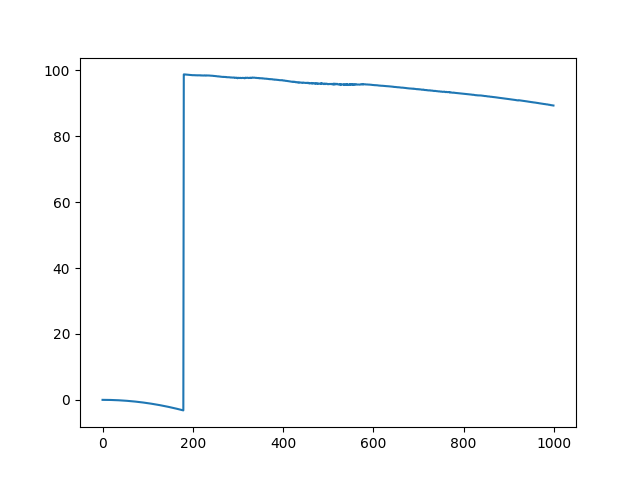
\includegraphics[width=12cm]{images/mountaincarcont.png}
    \caption{The x-axis represents the magnitude of the for applied to the car (multiplied by 1000) and the y-axis represents the average reward achieved using that magnitude.}
    \label{fig:mountain_car_cont}
\end{figure}

The simple and intuitive nature of this solution is further confirmation that GP is a suitable approach for solving (at least simple) RL environments. Another interesting feature of this program is its similarity to the solution for cart-pole, despite the differences between the environments. This is an indication that environments that share common characteristics (e.g. classic control environments) might be solvable using similar solutions.

\chapter{Pendulum}
After succeeding to generate simple, interpretable solutions for cart-pole and mountain-car, I wanted to choose an environment that (1) was similar enough to expect the same general approach to be fruitful, and (2) posed a challenge that the GP algorithm had not yet overcome. Pendulum (also known as the inverted pendulum problem) is another popular classic control RL benchmark that simulates a pendulum suspended from a frictionless pivot. In the initial state of the environment the angle of the pendulum is randomised. The goal is to swing it until it points upwards and then keep it steady for as long as possible. Interestingly, the mechanics of the problem are very similar to mountain-car, but with one important difference that makes it significantly more difficult to solve: the desired state of the environment (the pendulum pointing up, which is equivalent to the car standing on top of the hill) needs to, not only be reached, but maintained. Practically, this means that the agent has to combine two strategies: one for transitioning to that desired state and another one for maintaining it.

%%%%%%%%%%%%%%%%%%%%%%%%%%%
% 6.1 Environment Details %
%%%%%%%%%%%%%%%%%%%%%%%%%%%
\section{Environment Details}
The observation object for this environment consists of the trigonometric functions $sin(\theta)$ (\verb+sintheta+) and $cos(\theta)$ (\verb+costheta+), which on a high level describe the angle between the pendulum and the horizontal axis, and the angular velocity of the pendulum, $\dot\theta$ (\verb+thetadot+) which is a measure of how fast the pendulum is rotating. The sign of \verb+thetadot+ indicates whether the pendulum is rotating clockwise (negative) or anticlockwise (positive), while the signs of \verb+costheta+ and \verb+sintheta+ vary based on the spatial region the pendulum occupies. Notice that this allows for the environment space to be split into four quadrants based on the signs of these two quantities (figure \ref{fig:pendulum_quadrants}), an observation that proved very useful in conceptualising many aspects of the problem and interpreting the various solutions the algorithm generated. The action space is the range $[-2.0, 2.0]$ of floating-point numbers, which represent the force (torque) that is applied to control the pendulum's rotation. Finally, the reward comes in the form of a cost, which means the agent receives a negative reward at each time-step (the maximum is $0$) that is proportional to the angle of the pendulum, its angular velocity, and the torque applied to it (see the GitHub Wiki page\footnote{\url{https://github.com/openai/gym/wiki/Pendulum-v0}} for the precise equation for the reward). 

Therefore, the goal of the environment is to bring the pendulum to a vertical angle, and keep it there with minimum effort. Unlike the previous environments, the solution criteria here are unspecified, so the average reward of an agent that takes random actions ($\approx-1220$) was used as a reference point for measuring performance.

\begin{figure}[ht]
    \centering
    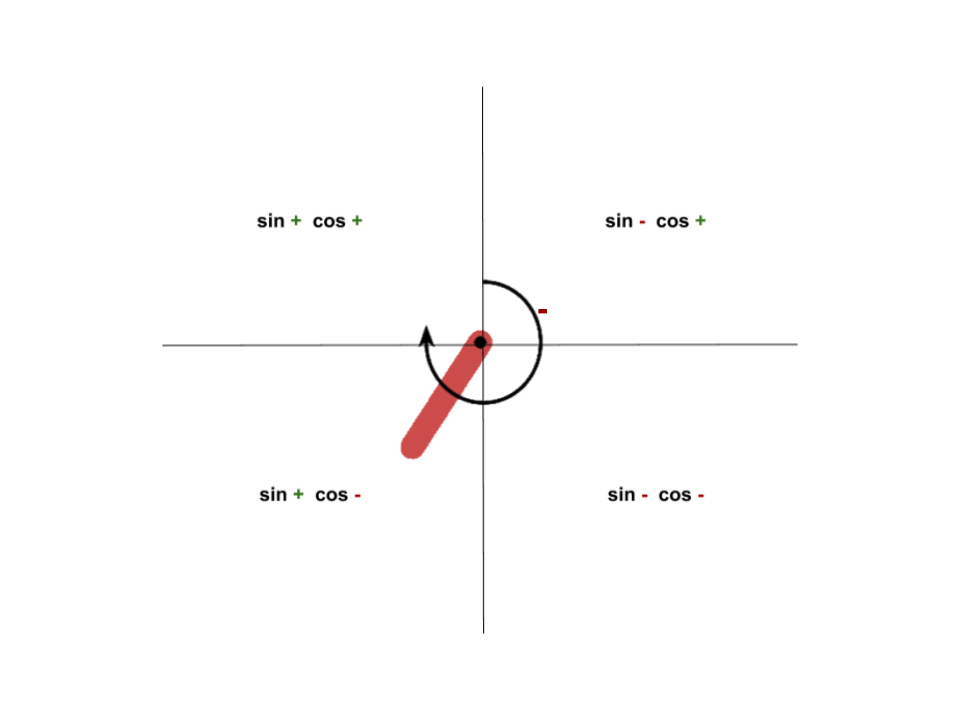
\includegraphics[width=12cm]{images/pendulum_quadrants.png}
    \caption{Visualisation of the signs of the pendulum observations}
    \label{fig:pendulum_quadrants}
\end{figure}

%%%%%%%%%%%%%%%%%%%%%%%%%%%%%%%%%%%%%
% 6.2 Experiment 1: Simple GP Agent %
%%%%%%%%%%%%%%%%%%%%%%%%%%%%%%%%%%%%%
\section{Experiment 1: Simple GP Agent}

% Setup %
\subsection{Setup and Motivation}
The main aim of the first experiment was to establish a performance baseline for the succeeding experiments to use as a reference point. Therefore, the program structure was simple, and similar to the one used in the previous environments:

\begin{verbatim}
F = {IFLTE}
T = {costheta, sintheta, thetadot, -1.0, 0.0, 1.0}
\end{verbatim}

The function set only includes the \verb+IFLTE+ function that proved very useful in solving the first two environments, and the terminal set includes all of the environment observations as well as three constants. The motivation behind the specific choice of constants was to allow the agent to draw decision boundaries around the observations (e.g. \verb+if costheta <= 0.0 and sintheta <= 0.0 then ...+) because a good strategy will probably need to make different decisions based on the angle of the pendulum. Since \verb+costheta+ and \verb+sintheta+ range over $[-1.0, 1.0]$, those limits were chosen as the constants, along with $0$ because it is reasonable to hypothesise that information about the sign of the observations is useful (for example the sign of \verb+thetadot+ can be used to determine whether the pendulum is rotating clockwise or anticlockwise).

The setup for this first experiment (summarised in table \ref{tab:pendulum_exp1_params}) followed that of the previous environments, with a few notable differences. Tournament selection was chosen instead of fitness proportionate selection, as discussed in Methods. Mutation was used for the first time to encourage exploration and avoid early convergence, both of which were not necessary in cart-pole and mountain-car. Notice, also, that while in the previous environments the terminal fitness was always the average reward required for a solution, the value used here was chosen more arbitrarily since pendulum has no specified solution criterion. Additionally, since pendulum has no episode termination criteria, the episode length had to be constrained explicitly. Finally, the number of episodes each program was run for to compute its fitness had to be decreased. The reason for this was, again, the absence of termination criteria: in cart-pole and mountain-car, even though the maximum episode length was 200 time-steps, most episodes did not run for that long, especially during the first few generations, because the programs failed quickly, causing the episodes to terminate prematurely. In pendulum, however, no such restriction exists, which meant that every program ran for the full episode length every time. As a result, the training time significantly increased, and it became impractical to run multiple experiments. The solution of reducing the number of episodes came at the cost of robustness because the fitness of each program became more sensitive to the randomisation of the initial environment state. This cost did not seem to be severe, however, since the experiment results showed a steady improvement in overall fitness from generation to generation. 

\begin{table}[ht]
    \centering
    \begin{tabular}{|l|c|}
        \hline
        \textbf{Parameters} & \textbf{Values} \\
        \hline
        Population size     & 200  \\
        Max generations     & 20   \\
        Terminal fitness & -200 \\
        Tournament size     & 10   \\
        Mutation rate       & 0.1  \\
        Max program depth   & 5    \\
        Number of runs      & 10   \\
        Number of episodes  & 10   \\
        Episode length      & 200  \\
        \hline
    \end{tabular}
    \caption{Experimental parameters (Pendulum Experiment 1)}
    \label{tab:pendulum_exp1_params}
\end{table}

% Results %
\subsection{Results and Discussion}
\subsubsection{Average Fitness Per Generation}
The average fitness the programs of each generation achieved is visualised in figure \ref{fig:pendulum_exp1_plot}. The first generation of programs performed very poorly, which was expected since they were randomly generated, but performance radically improved during the first four generations, before converging and remaining roughly the same for the remainder of the GP run. While the GP algorithm performed as expected, with each generation of programs performing better than the previous ones, it converged on a sub-optimal solution very quickly and showed no sign of improvement thereafter. Increasing the mutation rate delayed convergence and increased the variance in average fitness, but failed to make the algorithm escape the local minimum it appeared to be stuck on. These results gave rise to the hypothesis that the algorithm had discovered the best possible strategy given its current program structure, and failed to find a better solution because the program space was too restricted. Therefore, it was decided that the next experiment would introduce additional features to the language that could potentially be used to discover better solutions.

\begin{figure}[ht]
    \centering
    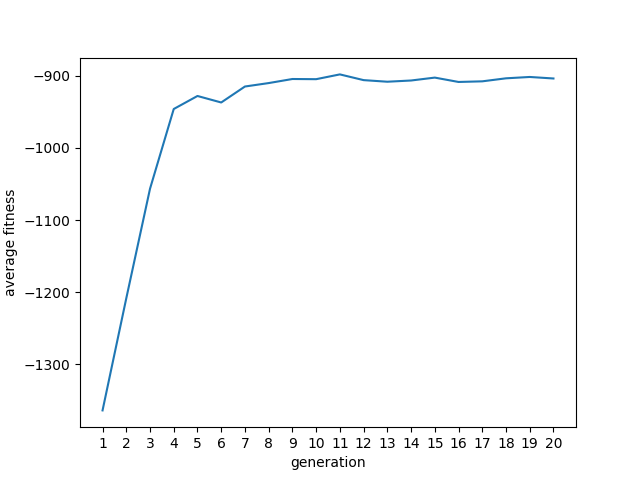
\includegraphics[width=12cm]{images/pend_simple_gp_agent.png}
    \caption{Average population fitness vs generations}
    \label{fig:pendulum_exp1_plot}
\end{figure}

\subsubsection{Best-Performing Programs}
At the end of each of the 10 runs of GP, the best-performing program, as well as the average reward (fitness) it achieved over 100 consecutive episodes, were recorded. The average fitness achieved by these programs was $-857$ and the programs themselves can be seen in table \ref{tab:pendulum_exp1_best_programs}. Looking at these programs, it quickly becomes obvious that most of them are identical or logically equivalent to the program \verb+IFLTE(thetadot, 0.0, costheta, 0.0)+. Additionally, it turned out that the programs that seem to be different due to their complexity (programs 3, 5, and 8 in the table) can also be reduced to this program. Therefore, the algorithm did not simply converge on various strategies with similar performance scores, but on syntactically equivalent programs that encoded a single strategy. This observation provided further evidence that the hypothesis regarding the limitations imposed by the program structure was correct.

\begin{table}[ht]
    \centering
    \begin{tabular}{|l|c|}
        \hline
        \multicolumn{1}{|c|}{\textbf{Programs}} & \textbf{Fitness} \\
        \hline
        
        \verb+IFLTE(thetadot, 0.0, costheta, 0.0)+ & -906  \\ \hline
        \verb+IFLTE(0.0, thetadot, 0.0, costheta)+ & -835  \\ \hline
        \verb+IFLTE(0.0, IFLTE(-1.0, 1.0, thetadot, sintheta), 0.0, costheta)+ & -884  \\ \hline
        \verb+IFLTE(thetadot, 0.0, costheta, 0.0)+ & -826  \\ \hline
        
        \verb+IFLTE(thetadot, 0.0, costheta,+ & \\
        \verb+  IFLTE(IFLTE(1.0, thetadot,+ & -833 \\
        \verb+  IFLTE(-1.0, 0.0, -1.0, thetadot), -1.0), -1.0, 0.0, thetadot))+ & \\
        \hline
        
        \verb+IFLTE(0.0, thetadot, 0.0, costheta)+ & -852  \\ \hline
        \verb+IFLTE(0.0, thetadot, 0.0, costheta)+ & -832  \\ \hline
        
        \verb+IFLTE(0.0, thetadot,IFLTE(costheta, 1.0,+ & \\
        \verb+  IFLTE(0.0, 1.0, 0.0, costheta),+ & -892 \\
        \verb+  IFLTE(0.0, -1.0, costheta, -1.0)), costheta)+ & \\
        \hline
        
        \verb+IFLTE(thetadot, 0.0, costheta, 0.0)+ & -868  \\ \hline
        \verb+IFLTE(0.0, thetadot, 0.0, costheta)+ & -842  \\ \hline
    \end{tabular}
    \caption{Best programs of each GP run (Pendulum Experiment 1)}
    \label{tab:pendulum_exp1_best_programs}
\end{table}

\subsubsection{Strategy Interpretation}
The program discovered by the GP algorithm, while not optimal, performed significantly better than a random agent, which made it a good starting point for tackling pendulum. It is, therefore, useful to discuss the interpretation of the strategy this program encodes to identify its limitations and justify the improvements implemented in the subsequent experiments. As noted in the environment description, the agent's goal is twofold: swing the pendulum until it's standing upright, and then keep it there with minimum effort. So, the strategy should be examined in terms of how well (or poorly) it performs with respect to these two sub-goals. 

The strategy encoded by this program is: "if the pendulum is rotating clockwise (negative angular velocity), then apply a torque to it that is equal to the cosine of its angle; otherwise, apply no torque to it at all." To understand this strategy, one needs to understand how \verb+costheta+ changes in the environment. As seen in figure \ref{fig:pendulum_quadrants}, \verb+costheta+ is negative in the bottom two quadrants, $0$ when the pendulum is parallel to the horizontal axis, and positive in the upper two quadrants. Therefore, concerning the first sub-goal, if the pendulum is rotating clockwise, a negative torque is applied to it, accelerating its clockwise rotation, whereas if the pendulum is rotating anticlockwise, it is let to swing freely. The result of this is that the pendulum is repeatedly pushed to rotate clockwise, then allowed to swing back freely, until it has built enough momentum to swing to the upper section of the screen. An interesting detail to note is that as the pendulum approaches a horizontal angle from the bottom quadrants, \verb+costheta+, and in turn the applied torque, tend to $0$. The effect of this is that the pendulum's momentum is great enough for it to reach an upright position, but not too great to cause it to be impossible to slow down (and, then, balance) once it has reached it. Finally, notice that this first half of the strategy is similar to the one discovered for mountain-car, where the car is pushed back-and-forth until it has enough momentum to climb the hill and reach the goal. This makes sense considering the similarity between the two environments discussed earlier.

It is clear that this strategy achieves the first sub-goal, but the difference to mountain-car is that the agent now has to use a different strategy to achieve the additional sub-goal of balancing the pendulum upright. When the pendulum enters the top-left quadrant, \verb+costheta+ becomes positive. Since \verb+thetadot+ is still negative at this point, this change causes the pendulum to slow down, as an opposite torque equal to \verb+costheta+ is applied to it. When \verb+thetadot+ is decreased to $0$ the else-branch of the if-statement encoded in the strategy takes effect and no torque is applied, preventing the pendulum to enter an anticlockwise rotation. The observed result is that the pendulum gradually slows down until it reaches the vertical position, then begins to speed up as it reaches the upper-right quadrant, and eventually falls to the bottom, letting the entire process repeat, with the only difference being that the pendulum has enough momentum now to not need to be swung back-and-forth to 'escape' the bottom quadrants.

\subsubsection{Problems and Ideas For Improvement}
This strategy solves the first sub-problem of escaping the bottom quadrants adequately and approximates a solution to the second sub-problem of keeping the pendulum standing upright by slowing it down and then applying no torque to it, which keeps it close to a vertical angle for some time and minimises the applied effort. The issue with this strategy is that, while the pendulum slows down, it doesn't stop once it reaches that vertical angle, so it inevitably falls to one side and keeps rotating.

It seemed that the current program structure should be sufficient to figure out an improvement for this strategy that addressed this issue. For example, a nested if-statement might be used to describe a new case where the pendulum is at a vertical angle and an action to take in that case, which would result in the desirable balancing behaviour. Additionally, as discussed above, it was reasonable to assume, based on the results, that the algorithm suffered from an early convergence problem that an extension to the program space might be able to improve. With this in mind, the second experiment was set up with a minor extension to the program structure and an encouragement of exploration in the form of an increase to the program depth and the maximum number of generations to evolve.

%%%%%%%%%%%%%%%%%%%%%%%%%%%%%%%%%
% 6.3 Experiment 2: Exploration %
%%%%%%%%%%%%%%%%%%%%%%%%%%%%%%%%%
\section{Experiment 2: Exploration}

% Setup %
\subsection{Setup and Motivation}
This experiment was intentionally very similar to experiment 1. As seen in table \ref{tab:pendulum_exp2_params}, most parameters were left unchanged with a few exceptions. Specifically, the terminal fitness was decreased from $-200$ to the theoretical maximum, $0$, in case this version of the agent managed to find an exceptionally good solution. More importantly, the maximum number of generations and the program depth were increased to encourage exploration by allowing the GP algorithm more time to generate more complex programs.

The program structure was also very similar, with only two additions that would hopefully allow for better strategies to emerge without reducing interpretability. The function \verb+neg+, which simply returns the opposite of a numerical input, was introduced to increase the number of combinations of observation values used without introducing completely new constructs. Secondly, a small constant ($0.25$) was added to the terminal set to give the agent an alternative value to use as an action. The motivation behind this last addition was that if one of the evolved strategies managed to balance the pendulum at a vertical angle, it would need to apply as small a torque as possible to minimise its effort. Finally, the constants $1.0$ and $-1.0$ were removed, since they didn't prove to be useful in the previous experiment.

\begin{table}[ht]
    \centering
    \begin{tabular}{|l|c|}
        \hline
        \textbf{Parameters} & \textbf{Values} \\
        \hline
        Population size     & 200  \\
        Max generations     & 30   \\
        Terminal fitness & 0 \\
        Tournament size     & 10   \\
        Mutation rate       & 0.1  \\
        Max program depth   & 10    \\
        Number of runs      & 5   \\
        Number of episodes  & 10   \\
        Episode length      & 200  \\
        \hline
    \end{tabular}
    \caption{Experimental parameters (Pendulum Experiment 1)}
    \label{tab:pendulum_exp2_params}
\end{table}

% Results %
\subsection{Results \& Discussion}
\subsubsection{Average Fitness Per Generation}
As seen in figure \ref{fig:pendulum_exp2_plot}, the average fitness followed a similar pattern to that of the previous experiment, starting very low and increasing rapidly in the first 4 generations. However, in this case, the algorithm did not converge on a single strategy at that point, but kept improving for the remainder of the run. This is an indication that expanding the program space had the desired effect of allowing the algorithm to escape the sub-optimal solution it was stuck on and discover better-performing strategies.

\begin{figure}[ht]
    \centering
    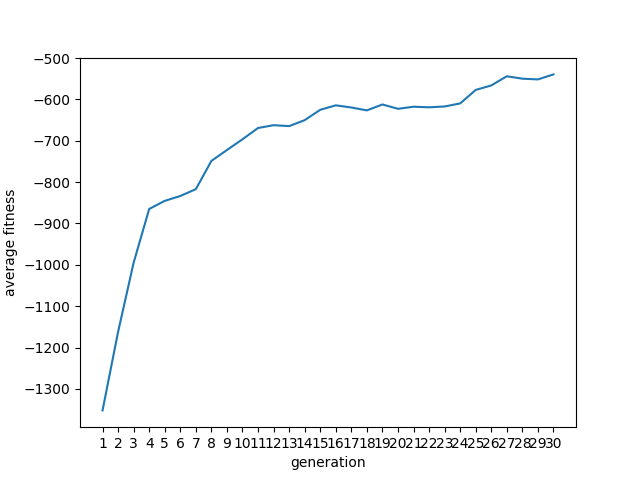
\includegraphics[width=12cm]{images/pendulum_deep_simple_GP.png}
    \caption{Average population fitness vs generations}
    \label{fig:pendulum_exp2_plot}
\end{figure}

\subsubsection{Best-Performing Programs}
While already visible in the average fitness graph, the best-performing programs of each GP run confirmed that the experiment was a success. The 5 generated programs, listed in table \ref{tab:pendulum_exp2_best_programs}, achieved an average fitness score of $-494.8$, almost half of what was achieved in the previous experiment, without an increase in complexity. Additionally, similarly to the previous experiment, all of these programs encode a single strategy which is easy to interpret. It is also interesting to note that the only useful modification to the program structure seems to have been the introduction of the \verb+neg+ function. Finally, increasing the population size and the number of maximum generations did not yield a better strategy, which is an indication that the algorithm had once again reached the limits allowed by the current program structure, so an improvement would probably require a language extension.

\begin{table}[ht]
    \centering
    \begin{tabular}{|l|c|}
        \hline
        \multicolumn{1}{|c|}{\textbf{Programs}} & \textbf{Fitness} \\
        \hline
        
        \verb+IFLTE(neg(sintheta), thetadot, neg(costheta), costheta)+ & -550  \\ \hline
        \verb+IFLTE(neg(sintheta), thetadot, neg(costheta), costheta)+ & -453  \\ \hline
        \verb+IFLTE(thetadot, neg(sintheta), costheta, neg(costheta))+ & -522  \\ \hline
        \verb+IFLTE(neg(thetadot), sintheta, neg(costheta), costheta)+ & -480  \\ \hline
        
        \verb+IFLTE(thetadot, IFLTE(0.25, 0.0,+ & \\
        \verb+  thetadot, neg(sintheta)), costheta,+ & -469 \\
        \verb+  IFLTE(costheta, costheta, neg(costheta), neg(0.0)))+ & \\
        \hline
    \end{tabular}
    \caption{Best programs of each GP run (Pendulum Experiment 2)}
    \label{tab:pendulum_exp2_best_programs}
\end{table}

\subsubsection{Strategy Interpretation}
All of the programs generated by the GP algorithm are identical or logically equivalent to the program \verb+IFLTE(thetadot, neg(sintheta), costheta, neg(costheta))+, which encodes the following strategy: "if \verb+thetadot+ $\leq$ -\verb+sintheta+ then apply a torque of magnitude \verb+costheta+; otherwise, apply a torque of magnitude -\verb+costheta+." Due to the mathematical nature of the description of the environment, this strategy does not seem intuitively interpretable. It is, therefore, useful to examine how this strategy causes the pendulum to behave in each of the four quadrants, as displayed in figure \ref{fig:pendulum_quadrants}. Additionally, it is useful to assess how well this strategy performs with respect to the two sub-goals that the agent needs to achieve: (1) rotate the pendulum until it reaches an upward vertical angle and (2) keep the pendulum balanced once it reaches that position.

With respect to (1), the two bottom quadrants are of interest. If the pendulum is in the bottom-right quadrant and \verb+thetadot+ $\leq$ \verb+-sintheta+ then \verb+thetadot+ is in $[-8.0, 1.0]$, which means the pendulum is either rotating clockwise, or it's rotating anticlockwise at a very low speed. In this case, the strategy applies a torque of magnitude \verb+costheta+, which is a negative value. If, however, the pendulum is in the bottom-right quadrant and is rotating anticlockwise at a high speed, apply a torque of magnitude \verb+-costheta+, which is a positive value. Therefore, in the bottom-right quadrant, the strategy says, if the pendulum is rotating clockwise, or anticlockwise but at a low speed, then push it clockwise, but if it's rotating anticlockwise at a high speed, then push it anticlockwise. This seems to be the most efficient way of making the pendulum swing up to the top quadrants, so this part of the strategy is reasonable. 

If the pendulum is in the bottom-left quadrant, a similar rule is applied. If \verb+thetadot+ $\leq$ -\verb+sintheta+ then \verb+thetadot+ is in $[-8.0, 0.0]$, which means the pendulum is rotating clockwise. In this case, the pendulum is pushed by \verb+costheta+, and therefore clockwise since \verb+costheta+ is negative, accelerating its current rotation so that it can reach the top quadrants. If \verb+thetadot+ $\geq$ -\verb+sintheta+ then \verb+thetadot+ is in [-1.0, 8.0], which means it's rotating anticlockwise or clockwise at a low speed. In this case, the pendulum is pushed by -\verb+costheta+, and therefore anticlockwise, which also accelerates its current rotation. Again, this seems to be the most efficient way to increase the pendulum's momentum enough to make it escape the bottom quadrants and achieve the first sub-goal.

With respect to (2), the top quadrants are considered. If the pendulum is in the top-left quadrant and \verb+thetadot+ $\leq$ -\verb+sintheta+ then the pendulum is rotating clockwise. In this case, the pendulum is pushed by \verb+costheta+, and therefore anticlockwise. This serves to slow the pendulum down, which is the desired behaviour here. If the pendulum is in the top-left quadrant and rotating anticlockwise, then it's pushed clockwise, bringing it towards the desired vertical angle. Similarly, in the top-right quadrant, if the pendulum is rotating clockwise (or anticlockwise but at a very low speed) then it is pushed anticlockwise, which pushes it towards the vertical angle, and if it is rotating anticlockwise, then it is pushed clockwise, which slows it down.

\section{Manual Improvement}
\subsection{Problem With Current Strategy}
The strategy generated as a result of experiment 2, seemed to behave effectively with respect to both sub-goals, in each of the four states (quadrants) that the pendulum might be in. This, then, begged the question, why this strategy could not achieve a better score. The first possible problem (confirmed by manual observation) was that the maximum value of \verb+costheta+ and -\verb+costheta+ (the two values used as the applied torque) were not large enough to slow down the pendulum when it was swung up to the top quadrants. So, if the agent failed to balance the pendulum on its first rotation, it would have accumulated too much momentum by the second rotation for the agent to be able to slow down and balance it. 

\subsection{Manual Intervention and Significance of Results}
This problem seemed simple to address: every occurrence of \verb+costheta+ could be replaced with \verb+costheta+ multiplied by some constant, to increase the torque applied to the pendulum, which would hopefully allow it to maintain its balance once it has reached a vertical angle. To test this hypothesis, a simple, brute-force optimisation procedure was implemented, which evaluated the strategy multiple times, each time multiplying \verb+costheta+ by a different constant (the range used was $[1.0, 10.0]$), and returned the constant that made the strategy perform the best. The result was surprisingly positive. The same strategy, modified to multiply the applied torque by $9.0$, consistently achieved an average reward of $\approx-200$ over 100 consecutive episodes. For comparison, the best neural-network-based solutions on the environment leaderboard page\footnote{\url{https://github.com/openai/gym/wiki/Leaderboard}} achieve an average reward of $\approx-123$. The following is the program that achieved this result: \\\verb+IFLTE(thetadot, neg(sintheta), costheta*9.0, neg(costheta*9.0))+.

This result was very significant because it is evidence of the potential benefits of interpretable solutions to RL problems. The only way to improve a neural network is by adjusting its parameters or architecture and re-training it. However, this case study is a good example of how interpretability can be useful because it allows manual intervention via logic and intuition to systematically modify and improve the solutions discovered automatically by algorithms. 

\subsection{Further Problems and Future Extensions}
A second problem that was identified was that, once the agent had managed to balance the pendulum, it put too much effort (torque) into keeping it balanced, so it accumulated a lot of negative reward. So, an improvement to this strategy could involve a nested if-statement that is used to detect when the pendulum has been stabilised at a vertical position, and then reduce the applied torque to a minimum. Such an improvement would probably require an extension to the program structure and quite a bit of exploration using the GP algorithm to discover a program that encodes this behaviour. 

\chapter{Conclusion}
All current state-of-the-art ML algorithms are black boxes with respect to the solutions they produce. Making those solutions interpretable is both a scientific and ethical imperative, as it will allow us to better understand and, thus, improve them while also making them more trustworthy. This project has achieved its aim of demonstrating, albeit at a small scale, that interpretability is both achievable and useful.

The first two environments tackled in this project, cart-pole and mountain-car, were relatively easy to find solutions for whereas pendulum posed more of a challenge. In all three cases, however, the combination of GP and human intervention was successful in producing simple, interpretable, and well-performing solutions. There is, of course, a lot of work that can still be done to improve the GP algorithm and extend the program structure to improve the current solutions. In particular, the experiments performed on pendulum as part of this project indicate that a few significant additions to the program structure could produce a solution that outperforms state-of-the-art neural-network-based approaches, so contributions to this (as well as to any other) part of the project are highly encouraged\footnote{The source code for this project can be found on GitHub under the MIT License: \url{https://github.com/alexgeorgousis/gp-for-interpretable-rl}}.

In principle, this approach could prove useful in solving more complicated RL environments, a task that could not be undertaken as part of this project due to time limitations. An environment like the OpenAI bipedal walker\footnote{\url{https://github.com/openai/gym/wiki/BipedalWalker-v2}} would be a reasonable next step following the progress made in this project, due to its similarity to the environments tackled here and the challenge the large amount of environmental inputs pose. The Atari games, which have become popular in RL research (see e.g. \cite{atari} and \cite{atari2}), and the MuJoCo environments\footnote{\url{https://gym.openai.com/envs/}}, which require algorithms to learn in a 3-D space, would also be interesting applications of this approach.

Finally, since this approach managed to yield solutions without a big trade-off in performance, a more rigorous comparison with neural-network-based approaches would be worth doing. Metrics such as training time, performance robustness, and code scalability are important to be measured and compared if this or similar approaches are to be used in industry.


\printbibliography

\end{document}
